\documentclass[crop,border=3pt]{standalone}
\usepackage[american,siunitx]{circuitikz}
\usetikzlibrary{arrows.meta,positioning,calc,fit}
\newcommand{\Cuk}{\mbox{\'{C}uk}}
\definecolor{stateblue}{RGB}{34,91,151}
\definecolor{stateorange}{RGB}{190,92,20}
\definecolor{softgray}{RGB}{244,245,247}
\begin{document}
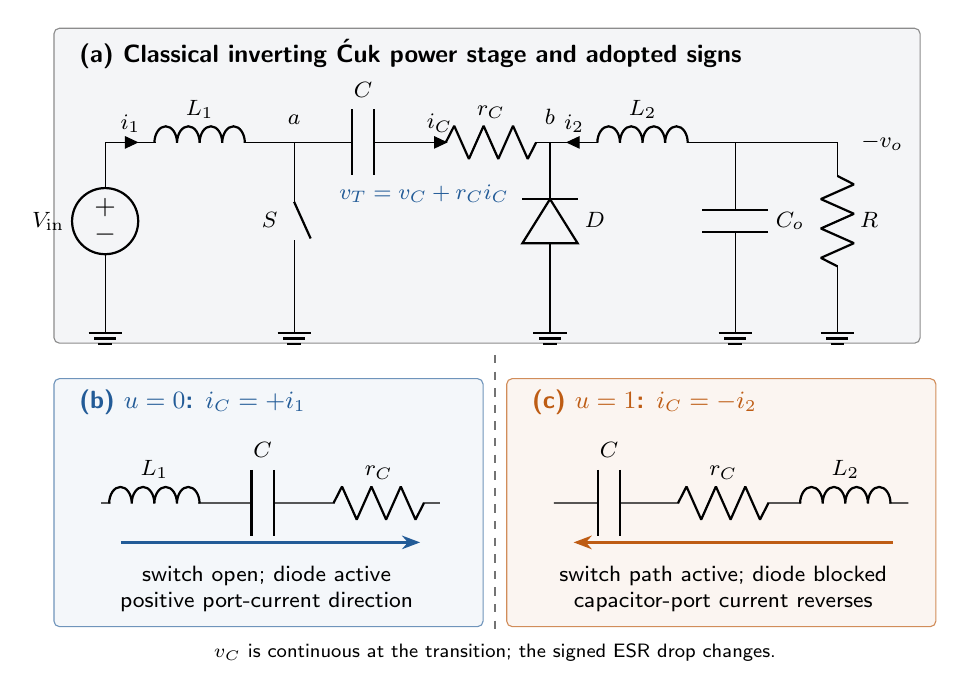
\begin{tikzpicture}[american currents,american voltages,
  every node/.style={font=\sffamily\footnotesize},
  flow/.style={-{Stealth[length=2.3mm]},line width=0.9pt}]
  % Full converter topology
  \draw[rounded corners=2pt,fill=softgray,draw=black!45]
    (-0.65,-0.55) rectangle (10.35,3.45);
  \node[font=\sffamily\bfseries\small,anchor=west] at (-0.45,3.12)
    {(a) Classical inverting \Cuk{} power stage and adopted signs};
  \draw (0,0) node[ground]{} to[V,invert,l=$V_{\mathrm{in}}$] (0,2)
    to[L,l=$L_1$,i>^=$i_1$] (2.4,2) coordinate (a)
    to[C,l=$C$] (4.15,2)
    to[R,l=$r_C$,i>^=$i_C$] (5.65,2) coordinate (b)
    to[L,l=$L_2$,i<^=$i_2$] (8.0,2) coordinate (o) -- (9.30,2);
  \draw (a) to[nos,l_=$S$] (2.4,0) node[ground]{};
  \draw (5.65,0) node[ground]{} to[D,l_=$D$] (b);
  \draw (o) to[C,l=$C_o$] (8.0,0) node[ground]{};
  \draw (9.30,2) to[R,l=$R$] (9.30,0) node[ground]{};
  \node[above=1mm] at (a) {$a$};
  \node[above=1mm] at (b) {$b$};
  \node[anchor=west] at (9.48,2) {$-v_o$};
  \node[stateblue,fill=softgray,inner sep=1.2pt] at (4.05,1.35)
    {$v_T=v_C+r_Ci_C$};

  % u=0 state panel
  \draw[rounded corners=2pt,fill=stateblue!5,draw=stateblue!65]
    (-0.65,-4.15) rectangle (4.80,-1.00);
  \node[font=\sffamily\bfseries\small,anchor=west,stateblue] at (-0.45,-1.30)
    {(b) $u=0$: $i_C=+i_1$};
  \draw (-0.05,-2.58) to[L,l=$L_1$] (1.30,-2.58)
    to[C,l=$C$] (2.70,-2.58) to[R,l=$r_C$] (4.25,-2.58);
  \draw[flow,stateblue] (0.20,-3.08) -- (4.0,-3.08);
  \node[align=center,text width=43mm] at (2.05,-3.67)
    {switch open; diode active\\positive port-current direction};

  % u=1 state panel
  \draw[rounded corners=2pt,fill=stateorange!6,draw=stateorange!70]
    (5.10,-4.15) rectangle (10.55,-1.00);
  \node[font=\sffamily\bfseries\small,anchor=west,stateorange] at (5.30,-1.30)
    {(c) $u=1$: $i_C=-i_2$};
  \draw (5.70,-2.58) to[C,l=$C$] (7.10,-2.58)
    to[R,l=$r_C$] (8.60,-2.58) to[L,l=$L_2$] (10.20,-2.58);
  \draw[flow,stateorange] (10.00,-3.08) -- (5.95,-3.08);
  \node[align=center,text width=43mm] at (7.85,-3.67)
    {switch path active; diode blocked\\capacitor-port current reverses};

  \draw[dashed,black!55,line width=0.7pt] (4.95,-0.70) -- (4.95,-4.25);
  \node[font=\sffamily\scriptsize,align=center] at (4.95,-4.48)
    {$v_C$ is continuous at the transition; the signed ESR drop changes.};
\end{tikzpicture}
\end{document}
